\section{Coordinate Systems}
\label{sec:coordinate}
\graphicspath{{_Intro/Figures/}}

\begin{figure}[!b]
	\centering
		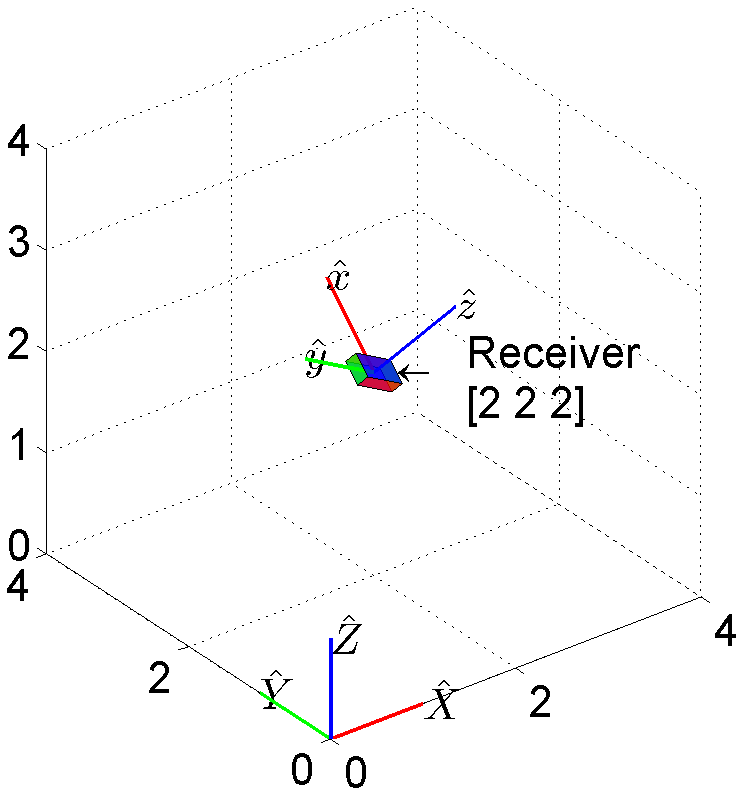
\includegraphics[width=3in]{figRcvrOrientation2.png}
	\caption{Illustration of the coordinate systems used}
	\label{fig:RcvrCoord}
\end{figure}

\figurename{ \ref{fig:RcvrCoord}} illustrates coordinate systems used in the analysis. [$\hat{\bf{X}}$ $\hat{\bf{Y}}$ $\hat{\bf{Z}}$] and [$\hat{\bf{x}}$ $\hat{\bf{y}}$ $\hat{\bf{z}}$] are the basis vectors for the GCS and the RCS. A corner of the room is the origin of the GCS while the center of the aperture of the receiver is set as the origin of RCS. The receiver's basis vectors are assumed always parallel to the length, width and surface normal of the sensor. 

Let [$x_{tx}$ $y_{tx}$ $z_{tx}$] be the location of centroid ($C_{tx}$) of the illumination surface of the transmitter and [$x_{rx}$ $y_{rx}$ $z_{rx}$] be the location of the centroid of the receiver concentrator surface in the GCS. The optical axis is then defined by ${\bf{d}}$ and the vertical distance between the transmitter and receiver is given by ${\bf{d}^{z}}$.

\begin{equation}
\label{eqOpAxis}
	{\bf{d}}=\vectthree{x_{tx}}{y_{tx}}{z_{tx}} - \vectthree{x_{rx}}{y_{rx}}{z_{rx}}
\end{equation}

\begin{equation}
\label{eqTxRxDist}
	{\bf{d}^{z}}=({\bf{d}}.{\hat{\bf{z}}}){\hat{\bf{z}}}
\end{equation}